
% This LaTeX was auto-generated from MATLAB code.
% To make changes, update the MATLAB code and republish this document.

\documentclass{article}
\usepackage{graphicx}
\usepackage{color}

\sloppy
\definecolor{lightgray}{gray}{0.5}
\setlength{\parindent}{0pt}

\begin{document}

    
    
\subsection*{Contents}

\begin{itemize}
\setlength{\itemsep}{-1ex}
   \item ELEC 4700 Assignment 4: Circuit Modeling
   \item Part 1
   \item DC Sweep
   \item AC Sweep
   \item Transient Circuit Simulation
   \item Part 2
   \item Introducing a Non-Linear Transconductance
\end{itemize}


\subsection*{ELEC 4700 Assignment 4: Circuit Modeling}

\begin{par}
Dilsha Appu-Hennadi, 101107857\newline Apr. 3, 2022 \newline Latest rev. Apr. 3, 2022
\end{par} \vspace{1em}
\begin{verbatim}
clear all
clearvars
clearvars -GLOBAL
close all
format shorte

global regL regW  nx ny L W

regL = 200e-9; % length of area
regW = 100e-9; % width of area

nx = 50; % number of space in x direction
ny = 50; % number of spaces in y direction

L = linspace(0, regL, nx); % nx spaces from 0 to region length
W = linspace(0, regW, ny); % ny spaces from 0 to region width

q = 1.60217662e-19; %C % elementary charge
m_e = 9.10938356e-31; %kg % rest mass of an electron
m_n = 0.26*m_e; %kg % mass of an electron
kb = 1.38064852e-23; %m^2 kg s^-2 K^-1 % Boltzmann's Constant

T = 300; %K % temperature

numElec = 800;%50;
numDispElec = 5;
t_mn = 0.2e-12; %s % mean time between collisions

numTimeStep = 800; %50;
dt = 1e-16;
\end{verbatim}


\subsection*{Part 1}

\begin{par}
The circuit shown in Figure 1 is the same circuit simulated in PA 7. However, this time there is no value for R3 given. Instead, a value for R3 will be determined through taking a voltage sweep of the bottle-neck simulation from Assignment 3, plotting the current-voltage characteristics, and taking the slope of a linear fit.
\end{par} \vspace{1em}
\begin{verbatim}
index = 1;

for V_0 = 0.1:0.1:10 % run voltage sweep

    icCharacteristics
    Voltage(index) = V_0;
    deviceCurrent(index) = Current;

    index = index + 1;

end

% conduct linear fit
p = polyfit(Voltage, deviceCurrent,1);
v = linspace(0.1,10,100);
c = polyval(p,v);

figure(1)
plot(Voltage, deviceCurrent, '*')
hold on
plot(v,c)
hold off
title('I-V Characteristics of R3')
xlabel('Voltage (V)')
ylabel('Current (A)')
legend('Data points', 'Linear fit')
\end{verbatim}

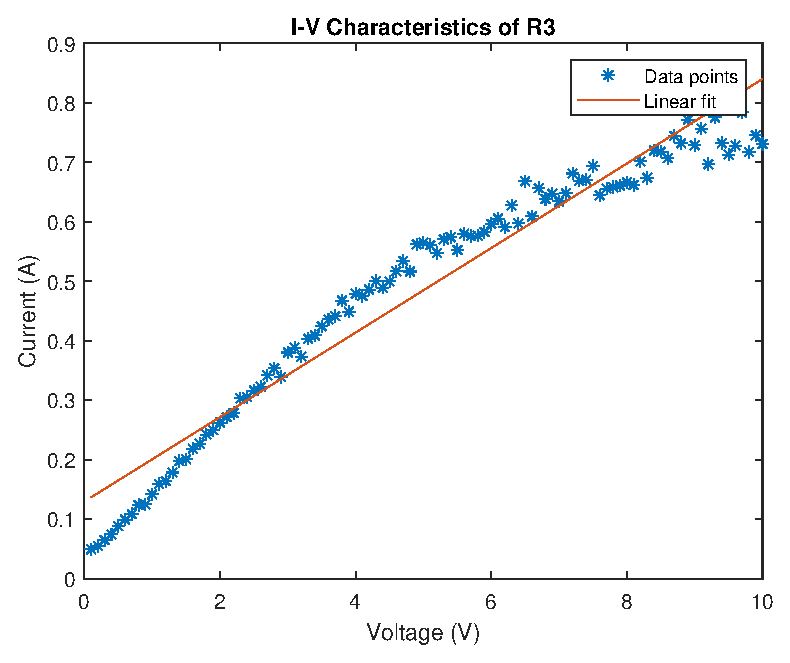
\includegraphics [width=4in]{main_01.eps}
\begin{par}
The figure above depicts the currents through R3 as voltage is swept from 0.1V to 10V using 0.1V increments. By plotting this data, we see that there is a clear linear relationship between the voltage and current through R3. By fitting the data to a 1st-order polynomial, we obtain the coefficients for a linear plot describing this relationship. A value for R3 can be obtained by taking the inverse of this slope such that:
\end{par} \vspace{1em}
\begin{par}
\[R3 = slope^{-1} = \left( \frac{I}{V} \right)^{-1} \approx 14 \Omega\]
\end{par} \vspace{1em}
\begin{par}
Below are the values for all components in the circuit:
\end{par} \vspace{1em}
\begin{verbatim}
V_in = 1;

R1 = 1
Cap = 0.25
R2 = 2
L_induct = 0.2
R3 = 1/p(1)
alpha = 100
R4 = 0.1
Ro = 1000

G1 = 1/R1
G2 = 1/R2
G3 = 1/R3
G4 = 1/R4
Go = 1/Ro
\end{verbatim}

        \color{lightgray} \begin{verbatim}
R1 =

     1


Cap =

   2.5000e-01


R2 =

     2


L_induct =

   2.0000e-01


R3 =

   1.4079e+01


alpha =

   100


R4 =

   1.0000e-01


Ro =

        1000


G1 =

     1


G2 =

   5.0000e-01


G3 =

   7.1026e-02


G4 =

    10


Go =

   1.0000e-03

\end{verbatim} \color{black}
    

\subsection*{DC Sweep}

\begin{par}
To begin analysis of the circuit, Kirchhoff's Current Law may be used to determine a set of differential equations that represent the network:
\begin{enumerate}
   \item \(I_{in} + G1V1 + C dV1/dt - G1V2 - C dV2/dt = 0\)
   \item \(-G1V1 - C dV1/dt + (G1 + G2))V2 + C dV2/dt + I_L = 0\)
   \item \(-I_L + I3 = 0\)
   \item \(-I + G4V4 - G4VO = 0\)
   \item \(-G4V4 + (G4+GO)VO = 0\)
   \item \(V1 = V_{in}\)
   \item \(- \alpha I3 + V4 = 0\)
   \item \(V2 - L dI_L/dt - R3I3 = 0\)
\end{enumerate}
\end{par} \vspace{1em}
\begin{par}
These equations can be writen in the frequency domain as well: \ensuremath{\backslash}[1\ensuremath{\backslash}:\ensuremath{\tilde{\;}}I\_\{in\} + G1V1 + Cj \ensuremath{\backslash}omega V1 - G1V2 - Cj \ensuremath{\backslash}omega V2 = 0\ensuremath{\backslash}] \ensuremath{\backslash}[2\ensuremath{\backslash}:\ensuremath{\tilde{\;}}-G1V1 - Cj \ensuremath{\backslash}omega V1 + (G1+G2)V2 + Cj \ensuremath{\backslash}omega V2 + I\_L = 0\ensuremath{\backslash}] \ensuremath{\backslash}[3\ensuremath{\backslash}:\ensuremath{\tilde{\;}}- I\_L + I3 = 0\ensuremath{\backslash}] \ensuremath{\backslash}[4\ensuremath{\backslash}:\ensuremath{\tilde{\;}}-I + G4V4 - G4VO = 0\ensuremath{\backslash}] \ensuremath{\backslash}[5\ensuremath{\backslash}:\ensuremath{\tilde{\;}}-G4V4 + (G4+GO)VO = 0\ensuremath{\backslash}] \ensuremath{\backslash}[6\ensuremath{\backslash}:\ensuremath{\tilde{\;}}V1 = V\_\{in\}\ensuremath{\backslash}] \ensuremath{\backslash}[7\ensuremath{\backslash}:\ensuremath{\tilde{\;}}- \ensuremath{\backslash}alpha I3 + V4 = 0\ensuremath{\backslash}] \ensuremath{\backslash}[8\ensuremath{\backslash}:\ensuremath{\tilde{\;}}V2 - Lj \ensuremath{\backslash}omega I\_L - R3I3 = 0\ensuremath{\backslash}]
\begin{enumerate}
   \item \(I_{in} + G1V1 + Cj \omega V1 - G1V2 - Cj \omega V2 = 0\)
   \item \(-G1V1 - Cj \omega V1 + (G1 + G2))V2 + Cj \omega V2 + I_L = 0\)
   \item \(-I_L + I3 = 0\)
   \item \(-I + G4V4 - G4VO = 0\)
   \item \(-G4V4 + (G4+GO)VO = 0\)
   \item \(V1 = V_{in}\)
   \item \(- \alpha I3 + V4 = 0\)
   \item \(V2 - Lj \omega I_L - R3I3 = 0\)
\end{enumerate}
\end{par} \vspace{1em}
\begin{par}
Our unknowns are: X = [I\_in, V1, V2, I\_L, I3, I, V4, Vo];
\end{par} \vspace{1em}
\begin{verbatim}
X = [];

G = zeros(8);
G(1,:) = [1 G1 -G1 0 0 0 0 0];
G(2,:) = [0 -G1 (G1+G2) 1 0 0 0 0];
G(3,:) = [0 0 0 -1 1 0 0 0];
G(4,:) = [0 0 0 0 0 -1 G4 -G4];
G(5,:) = [0 0 0 0 0 0 -G4 (G4+Go)];
G(6,:) = [0 1 0 0 0 0 0 0];
G(7,:) = [0 0 0 0 -alpha 0 1 0];
G(8,:) = [0 0 1 0 -R3 0 0 0];

C = zeros(8);
C(1,:) = [0 Cap -Cap 0 0 0 0 0];
C(2,:) = [0 -Cap Cap 0 0 0 0 0];
C(8,:) = [0 0 0 -L_induct 0 0 0 0];

F = [0 0 0 0 0 V_in 0 0];
\end{verbatim}
\begin{par}
Thus our C and G matricies are:
\end{par} \vspace{1em}
\begin{verbatim}
C

G
\end{verbatim}

        \color{lightgray} \begin{verbatim}
C =

  Columns 1 through 6

            0   2.5000e-01  -2.5000e-01            0            0            0
            0  -2.5000e-01   2.5000e-01            0            0            0
            0            0            0            0            0            0
            0            0            0            0            0            0
            0            0            0            0            0            0
            0            0            0            0            0            0
            0            0            0            0            0            0
            0            0            0  -2.0000e-01            0            0

  Columns 7 through 8

            0            0
            0            0
            0            0
            0            0
            0            0
            0            0
            0            0
            0            0


G =

  Columns 1 through 6

   1.0000e+00   1.0000e+00  -1.0000e+00            0            0            0
            0  -1.0000e+00   1.5000e+00   1.0000e+00            0            0
            0            0            0  -1.0000e+00   1.0000e+00            0
            0            0            0            0            0  -1.0000e+00
            0            0            0            0            0            0
            0   1.0000e+00            0            0            0            0
            0            0            0            0  -1.0000e+02            0
            0            0   1.0000e+00            0  -1.4079e+01            0

  Columns 7 through 8

            0            0
            0            0
            0            0
   1.0000e+01  -1.0000e+01
  -1.0000e+01   1.0001e+01
            0            0
   1.0000e+00            0
            0            0

\end{verbatim} \color{black}
    \begin{par}
With matrices C G and vector, F, determined, we can run a DC sweep with voltage, \(V_{in}\) sweeping from -10V to 10V. This can be done using the frequency domain equations with \(\omega = 0\).
\end{par} \vspace{1em}
\begin{verbatim}
DCsweep
\end{verbatim}

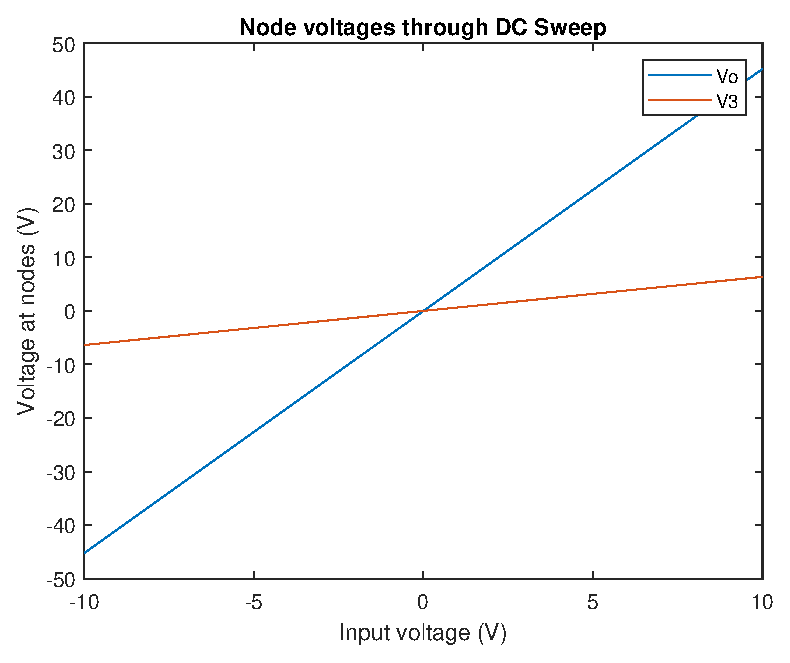
\includegraphics [width=4in]{main_02.eps}
\begin{par}
In Figure 2 above, we can see how the voltages V3 and VO change through the voltage sweep. Both voltages vary linearly as the input voltage increases. Since VO is dependent on \(\alpha I3\), it makes sense that if V3 is linear than VO must be linear. We also see that the slope of VO is steeper than V3, indicating that the signal is being amplified by the device.
\end{par} \vspace{1em}


\subsection*{AC Sweep}

\begin{par}
Similarly, we can also conduct a frequency sweep. To do this, we hold \(V_{in}\) at 1V then loop through different frequency values. VO and V3 are plotted with the change in frequency. The gain, in dB, can also be plotted.
\end{par} \vspace{1em}
\begin{verbatim}
ACsweep
\end{verbatim}

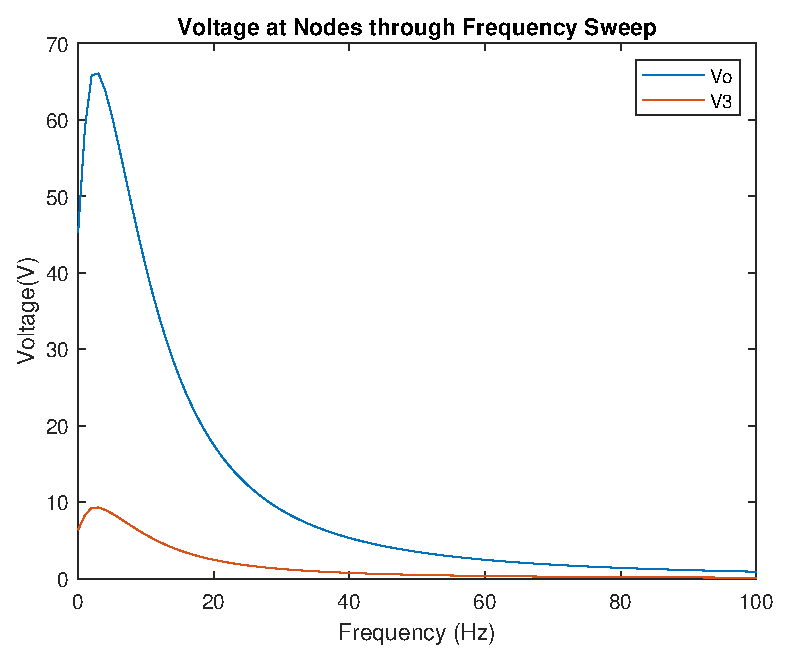
\includegraphics [width=4in]{main_03.eps}

\includegraphics [width=4in]{main_04.eps}
\begin{par}
We can also add some random perturbations to the capacitor to simulate a variable capacitor. For this, the standard deviation is assumed to be 0.05 and the frequency is assumed as \(\omega = \pi\).
\end{par} \vspace{1em}
\begin{verbatim}
Cperturb
\end{verbatim}

\includegraphics [width=4in]{main_05.eps}

\includegraphics [width=4in]{main_06.eps}


\subsection*{Transient Circuit Simulation}

\begin{par}
Looking back at the circuit depicted in Figure 1 of the assignment instructions, given the components within the circuit and their configuration, it seems that the circuit being modelled is a filter in series with an amplifier. Where R1 and C seem to model a capacitor with a lossy dielectric. This capacitor along with R2 and L would create a bandpass filter. R3, the current dependent voltage source and R4 would model the transistor amplifier and RO is the load.
\end{par} \vspace{1em}
\begin{par}
As mentioned earlier, as this circuit has both a capacitor and inductor, we can expect to see a bandpass type behaviour as both the capacitor and inductor will have an associateed cut-off frequency.
\end{par} \vspace{1em}
\begin{par}
In the time domain, the circuit can be represented by the equation:
\end{par} \vspace{1em}
\begin{par}
\[C \frac{dV}{dt} + GV = F\]
\begin{par}
   As a first order ODE this equation is a bit difficult to solve as it currently is. Instead, we can write it in its finite difference form and determine a numerical solution.
\end{par} \vspace{1em}
\[C \frac{V(t) - V(t - \Delta t)}{\Delta t} + G V(t) = F\]
\[\frac{C}{\Delta t}V(t) - \frac{C}{\Delta t}V(t - \Delta t) + GV(t) = F\]
\[V(t) = \left[ F + \frac{C}{\Delta t}V(t - \Delta t) \right] \left[ \frac{C}{\Delta t} + G \right]^{-1}\]
\end{par} \vspace{1em}
\begin{par}
For the purposes of the FDTD, we will use 1000 times steps to simulate 1 second - i.e. each time step will be a milisecond. Three different inputs will be used:
\end{par} \vspace{1em}
\begin{itemize}
   \item A unit step that steps up from 0V to 1V a 0.03 seconds.
   \item A sinusoid, first with a frequency of 1/0.03 Hz and another with a frequency of 10Hz.
   \item A Gaussian pulse with a magnitude of 1 and std. dev. of 0.03, after a delay of 0.06 seconds.
\end{itemize}
\begin{par}
   It should also be noted, that as previous values are being used in the calculation, all initial values will be assumed to be 0.
\end{par} \vspace{1em}
\begin{verbatim}
numSteps = 1000;
dt = 1e-3; %50e-3;

UnitStep
\end{verbatim}

        \color{lightgray} \begin{verbatim}Warning: Imaginary parts of complex X and/or Y arguments ignored. 
Warning: Imaginary parts of complex X and/or Y arguments ignored. 
\end{verbatim} \color{black}
    
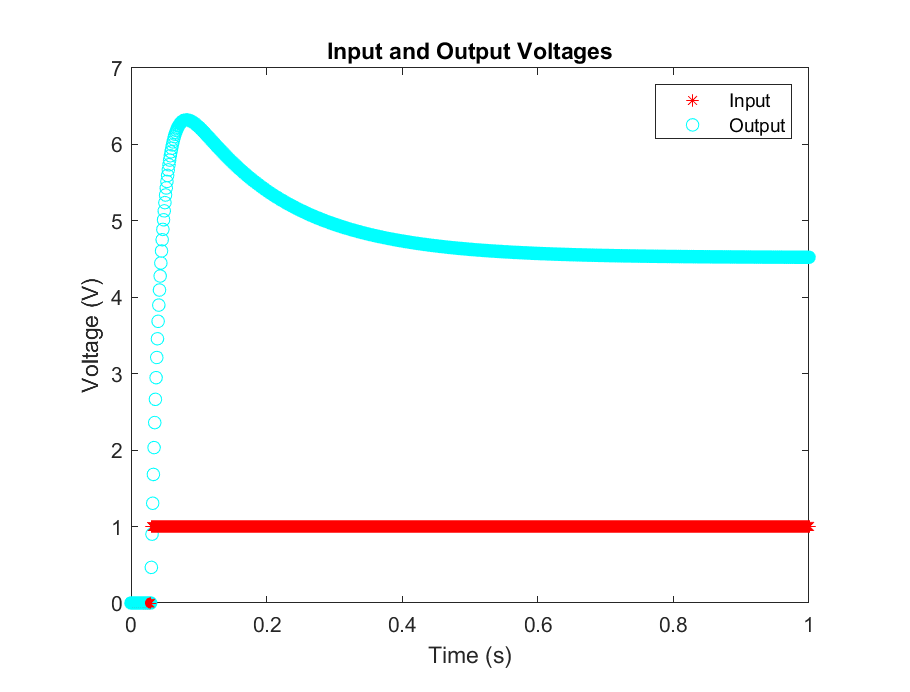
\includegraphics [width=4in]{main_07.eps}

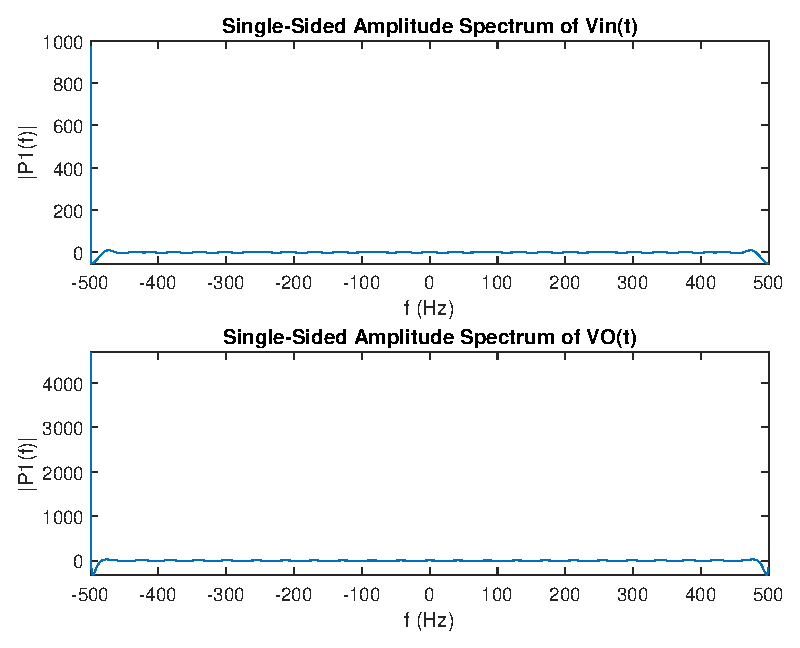
\includegraphics [width=4in]{main_08.eps}

\includegraphics [width=4in]{main_09.eps}
\begin{par}
Figure 7, above, depicts the input and output signals of the circuit over time. The input signal, which is a unit step at 0.06s, starts at 0V and at t = 0.06s, the signal jumps to 1V. This causes a transient response in the graph as the output tries to catch up to the input resulting in an overshoot which decreases and settles off at a final value after some time. As we saw earlier in the DC sweep graphs the output signal has a much larger amplitude than the input signal as the circuit amplifies the input.
\end{par} \vspace{1em}
\begin{par}
Figure 8 and 9 show the single-sided amplitude spectrum and the two-sided spectrum respectively. As the unit step is mainly a jump at some time t, we only see a single delta function within the amplitude spectrum graphs for both signals.
\end{par} \vspace{1em}
\begin{verbatim}
Sinusoid
\end{verbatim}

        \color{lightgray} \begin{verbatim}Warning: Imaginary parts of complex X and/or Y arguments ignored. 
Warning: Imaginary parts of complex X and/or Y arguments ignored. 
\end{verbatim} \color{black}
    
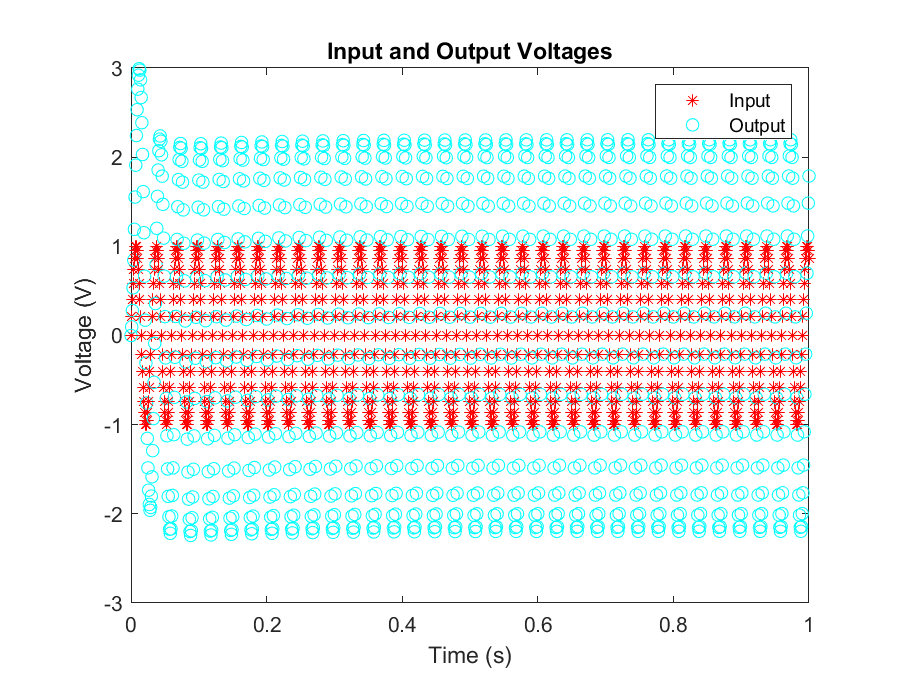
\includegraphics [width=4in]{main_10.eps}

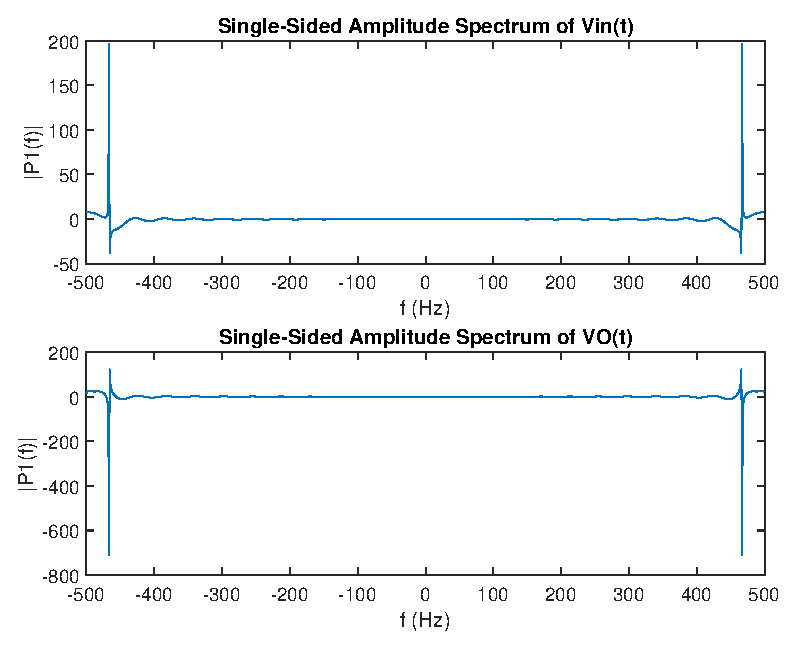
\includegraphics [width=4in]{main_11.eps}

\includegraphics [width=4in]{main_12.eps}
\begin{par}
Figures 10 shows the input and output wave forms of the circuit when a sinusoidal excitations is used. This input sinusiod has an amplitude of 1 and a frequency of about 33.33Hz. The output response from the circuit overshoots at the beginning as the circuit rushes to catch up to the input but quickly levels out at a steady state. Once again, we see the amplitude of the output is larger than the input, indicating an amplification of the input signal.
\end{par} \vspace{1em}
\begin{par}
Figure 11 is the single-sided amplitude spectrum, while Figure 12 is the two-siedd spectrum. While it's a bit unclear in Figure 11, Figure 12 indicates the frequency of both the input and output as about 33Hz, which is to be expected.
\end{par} \vspace{1em}
\begin{verbatim}
SinusoidV2
\end{verbatim}

        \color{lightgray} \begin{verbatim}Warning: Imaginary parts of complex X and/or Y arguments ignored. 
Warning: Imaginary parts of complex X and/or Y arguments ignored. 
\end{verbatim} \color{black}
    
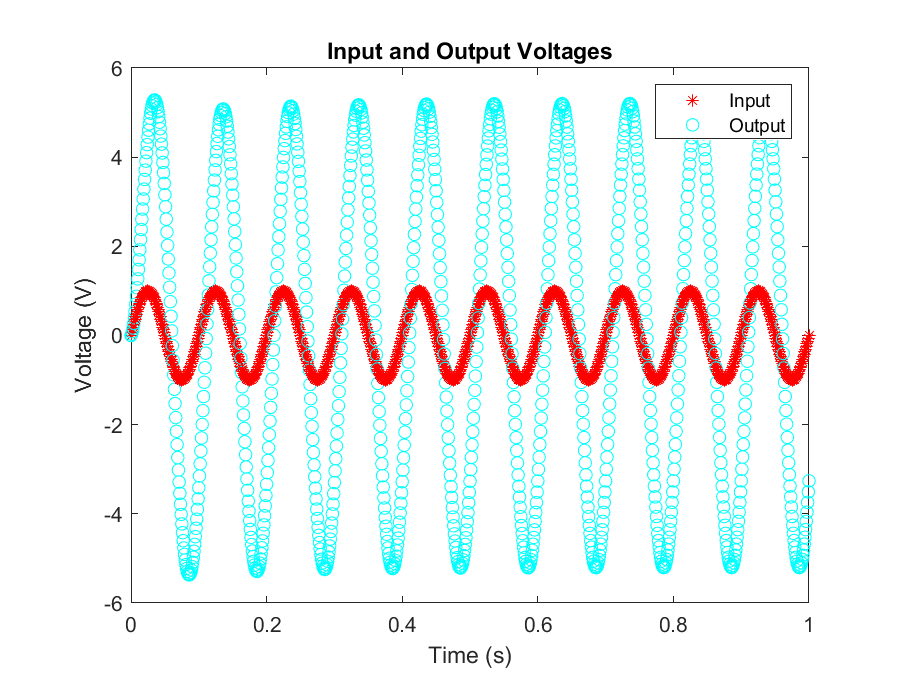
\includegraphics [width=4in]{main_13.eps}

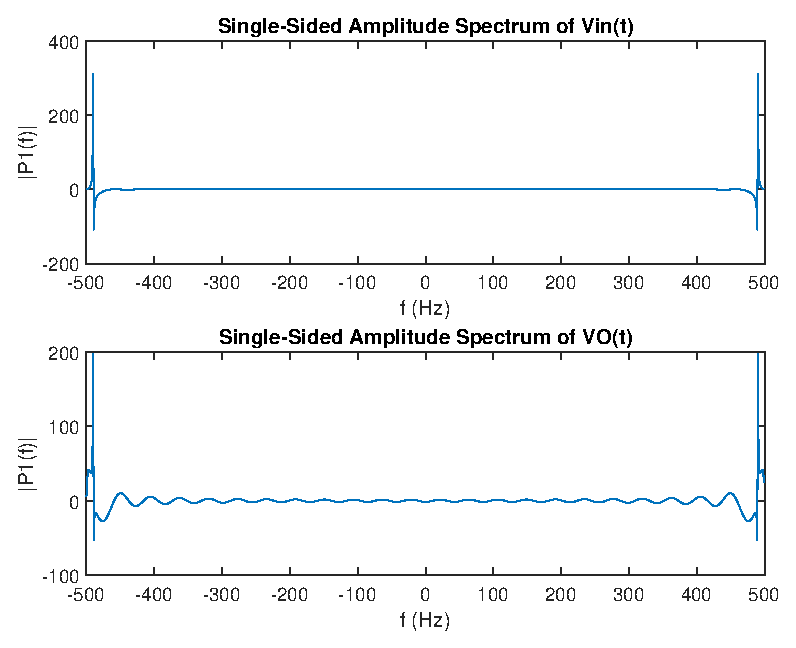
\includegraphics [width=4in]{main_14.eps}

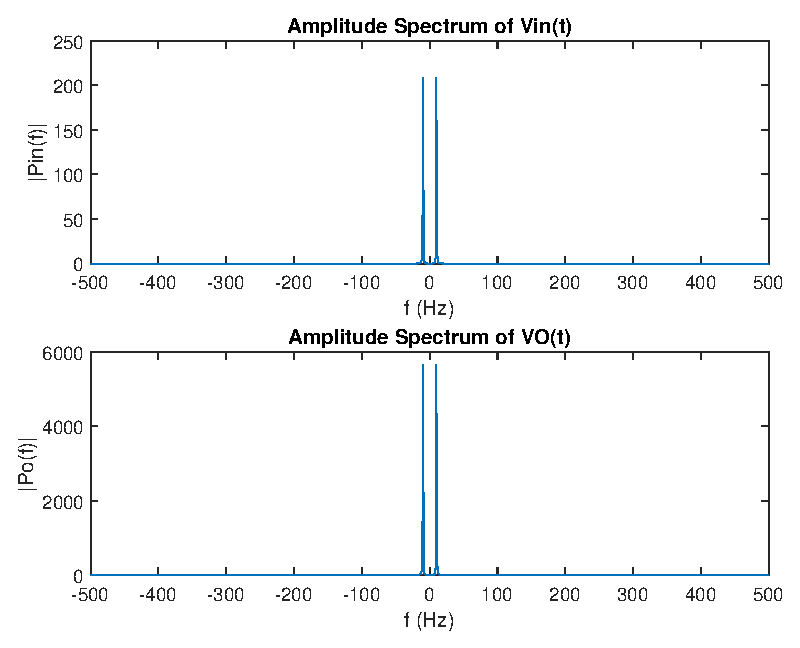
\includegraphics [width=4in]{main_15.eps}
\begin{par}
Figures 13 to 15 depict a similar situation to the previous excitation. This time, however, the sinusoid has a frequency of 10Hz. The lower frequency allows us to see the signals more clearly and we also see that there is a delay between the input and the output as the peaks/troughs of the two singnals do not occur at the same time.
\end{par} \vspace{1em}
\begin{par}
Additionally, looking at the results of the fft in Figures 14 and 15, the frequency of the input and output is found to be about 10Hz. This is what we expect it to be.
\end{par} \vspace{1em}
\begin{verbatim}
GaussianPulse
\end{verbatim}

        \color{lightgray} \begin{verbatim}Warning: Imaginary parts of complex X and/or Y arguments ignored. 
Warning: Imaginary parts of complex X and/or Y arguments ignored. 
\end{verbatim} \color{black}
    
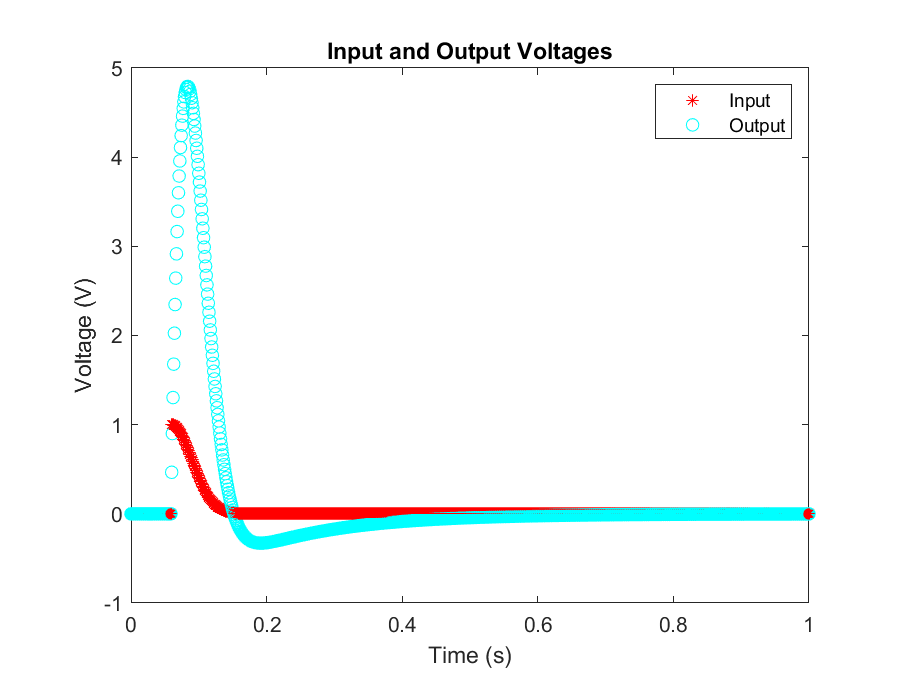
\includegraphics [width=4in]{main_16.eps}

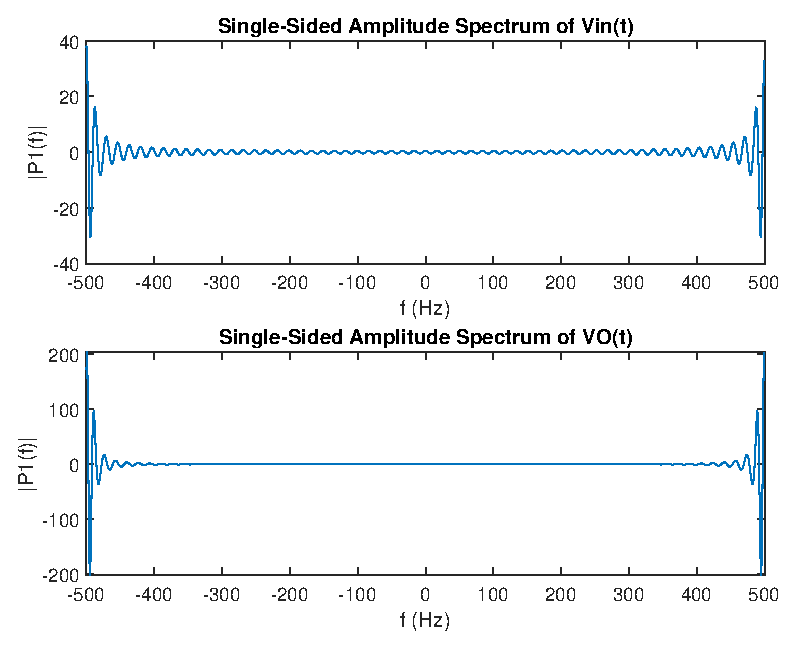
\includegraphics [width=4in]{main_17.eps}

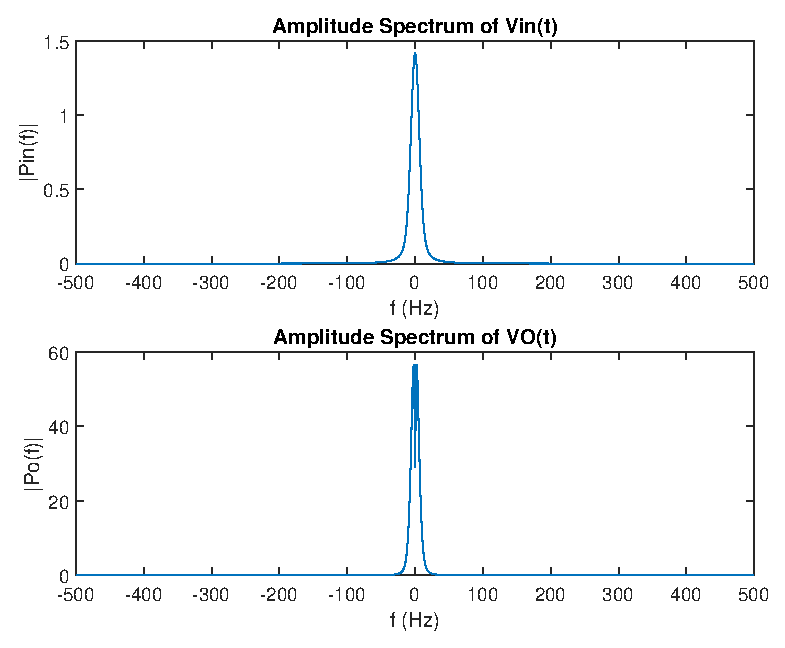
\includegraphics [width=4in]{main_18.eps}
\begin{par}
Figure 16 depicts the input Gaussian excitation and the corresponding output from the circuit. As seen earlier, there is a delay in the output. Then, after the Gaussian pulse ends, the output overshoots and dips below 0V before settle out to its steady state of 0V.
\end{par} \vspace{1em}
\begin{par}
From the FFT of the signals, the frequency seems to be about 2Hz
\end{par} \vspace{1em}
\begin{par}
So far the FFTs of the signals have been reasonably accurate to the fequency expected. However, as the step time, dt, is increased, we see the FFTs become less accurate.
\end{par} \vspace{1em}
\begin{par}
We can think of the step time as the period of the sampling frequency - i.e.: \(f_s = \frac{1}{dt}\). So we see, as the step time increases the sampling frequency decreases. According to the Nyquist-Shannon Sampling Theorem, in order to recreate a signal from a samples of the original signal, the sampling frequency must be more than double the frequency of the original signal: \[f < 2f_s\]
\end{par} \vspace{1em}


\subsection*{Part 2}

\begin{par}
For this part, the previous circuit is now slightly modified. It now includes a current source, \(I_n\) to model thermal noise and a capacitor, \(C_n\), to bandwidth limit the noise. With these additions, we must make some slight modifications to our set of equations:
\end{par} \vspace{1em}
\begin{enumerate}
   \item \(I_{in} + G1V1 + C dV1/dt - G1V2 - C dV2/dt = 0\)
   \item \(-G1V1 - C dV1/dt + (G1 + G2))V2 + C dV2/dt + I_L = 0\)
   \item \(-I_L + G3V3 + I_n + C_n dV3/dt = 0\)
   \item \(-I + G4V4 - G4VO = 0\)
   \item \(-G4V4 + (G4+GO)VO = 0\)
   \item \(V1 = V_{in}\)
   \item \(- \alpha G3V3 + V4 = 0\)
   \item \(V2 - L dI_L/dt - V3 = 0\)
\end{enumerate}
\begin{par}
The frequency domain equations can then be written as:
\end{par} \vspace{1em}
\begin{enumerate}
   \item \(I_{in} + G1V1 + Cj \omega V1 - G1V2 - Cj \omega V2 = 0\)
   \item \(-G1V1 - Cj \omega V1 + (G1 + G2))V2 + Cj \omega V2 + I_L = 0\)
   \item \(-I_L + G3V3 + I_n + C_nj \omega V3 = 0\)
   \item \(-I + G4V4 - G4VO = 0\)
   \item \(-G4V4 + (G4+GO)VO = 0\)
   \item \(V1 = V_{in}\)
   \item \(- \alpha G3V3 + V4 = 0\)
   \item \(V2 - Lj \omega I_L - V3 = 0\)
\end{enumerate}
\begin{par}
Our unknowns are: X = [I\_in, V1, V2, I\_L, V3, I, V4, Vo];
\end{par} \vspace{1em}
\begin{verbatim}
V_in = 1;
C_n = 0.00001;
I_n = rand;

X = [];

G = zeros(8);
G(1,:) = [1 G1 -G1 0 0 0 0 0];
G(2,:) = [0 -G1 (G1+G2) 1 0 0 0 0];
G(3,:) = [0 0 0 -1 G3 0 0 0];
G(4,:) = [0 0 0 0 0 -1 G4 -G4];
G(5,:) = [0 0 0 0 0 0 -G4 (G4+Go)];
G(6,:) = [0 1 0 0 0 0 0 0];
G(7,:) = [0 0 0 0 -alpha*G3 0 1 0];
G(8,:) = [0 0 1 0 -1 0 0 0];

C = zeros(8);
C(1,:) = [0 Cap -Cap 0 0 0 0 0];
C(2,:) = [0 -Cap Cap 0 0 0 0 0];
C(3,:) = [0 0 0 0 C_n 0 0 0];
C(8,:) = [0 0 0 -L_induct 0 0 0 0];

F = [0 0 -I_n 0 0 V_in 0 0];
\end{verbatim}
\begin{par}
We can once again use a FDTD numerical approach to simulate the circuit using a Gaussian excitation. The thermal noise can be simulated using a random numbers from a Gaussian distribution witha a mean of 0.001A.
\end{par} \vspace{1em}
\begin{verbatim}
Circ2Sim
\end{verbatim}

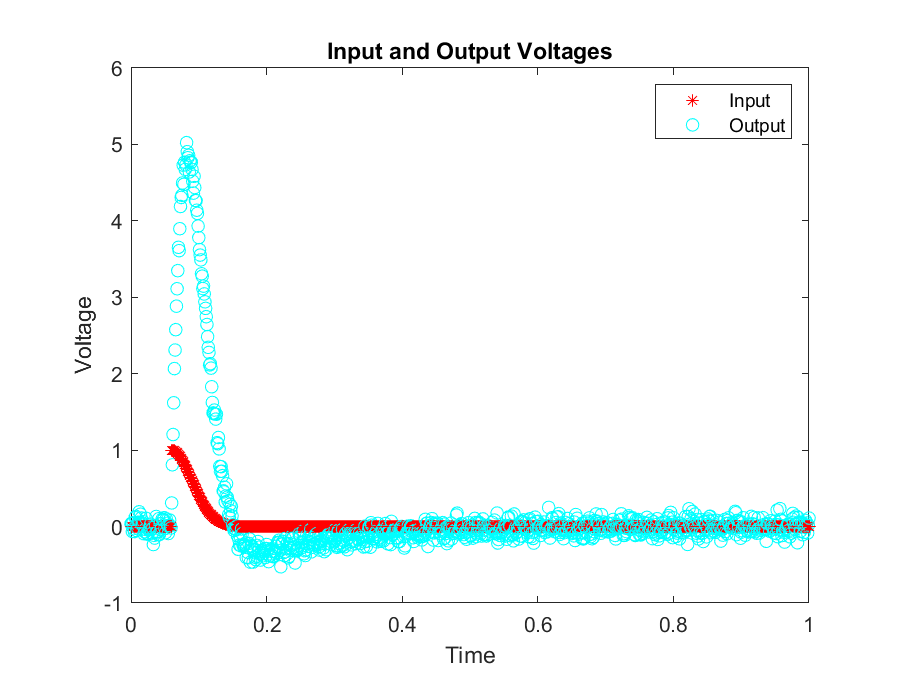
\includegraphics [width=4in]{main_19.eps}

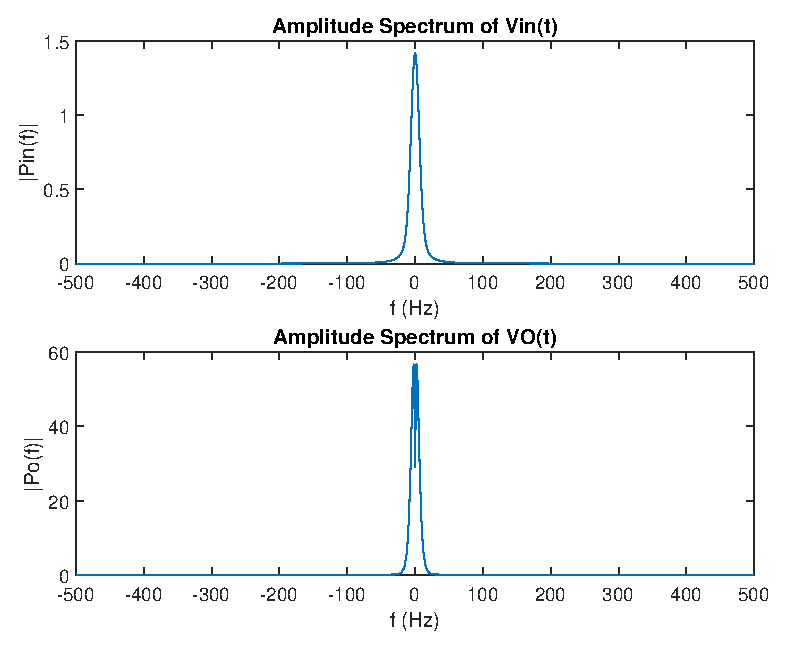
\includegraphics [width=4in]{main_20.eps}
\begin{par}
The plot in Figure 19 is similar to Figure 16, however, the output signal is noisier due to the inclusion of In. The FFT plot in Figure 20, on the other hand, still appears to be the sam as the FFT plot in Figure 18 (for the Gaussian excitations without noise). This is likely because the computation for the FFT is able to filter out the noise in the signal to isolate the actual ferquency of the signal.
\end{par} \vspace{1em}
\begin{par}
Next, we may vary Cn and observe the bandwidth to see how it affects the frequency response of the circuit.
\end{par} \vspace{1em}
\begin{verbatim}
figNum = 21;

for C_n = [1e-15 1e-6 1]

    C(3,:) = [0 0 0 0 C_n 0 0 0];

    VaryCn

    figNum = figNum + 1;

end
\end{verbatim}

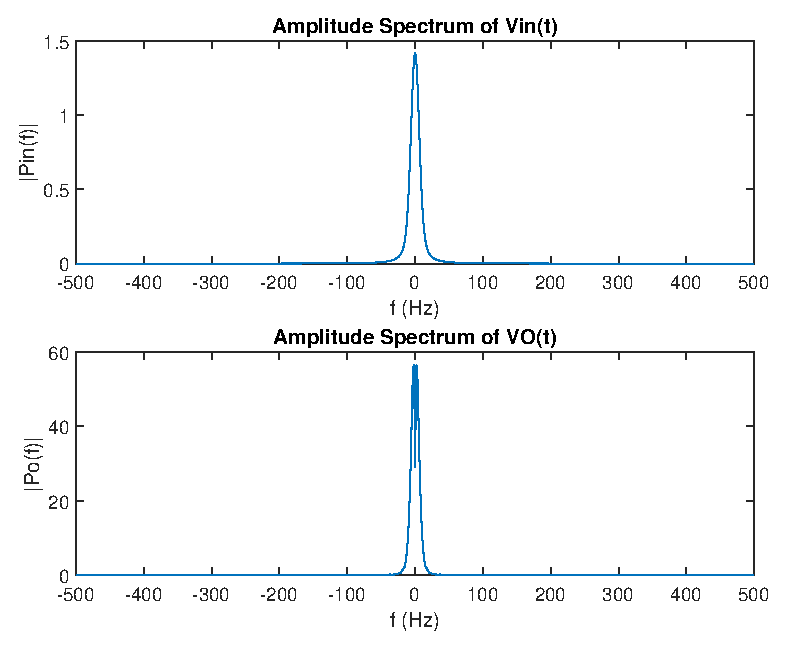
\includegraphics [width=4in]{main_21.eps}

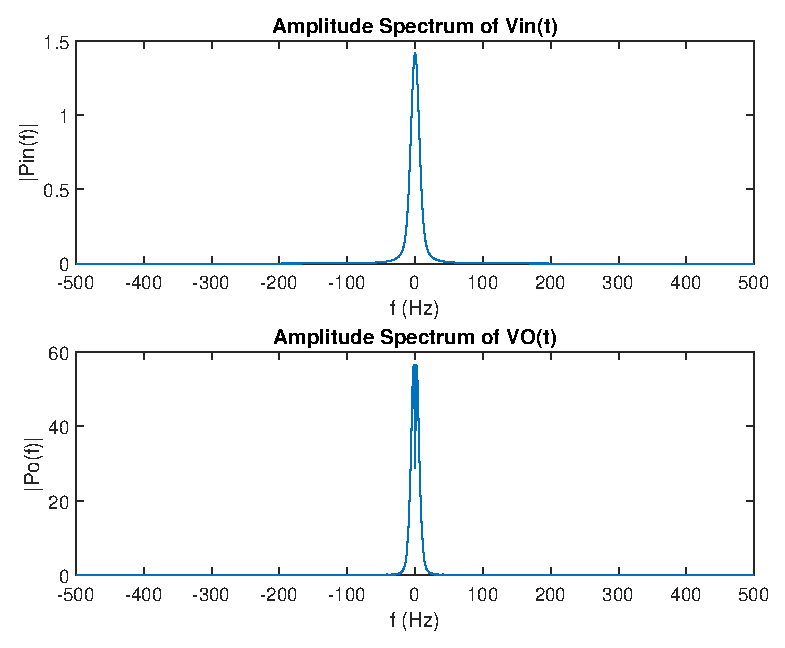
\includegraphics [width=4in]{main_22.eps}

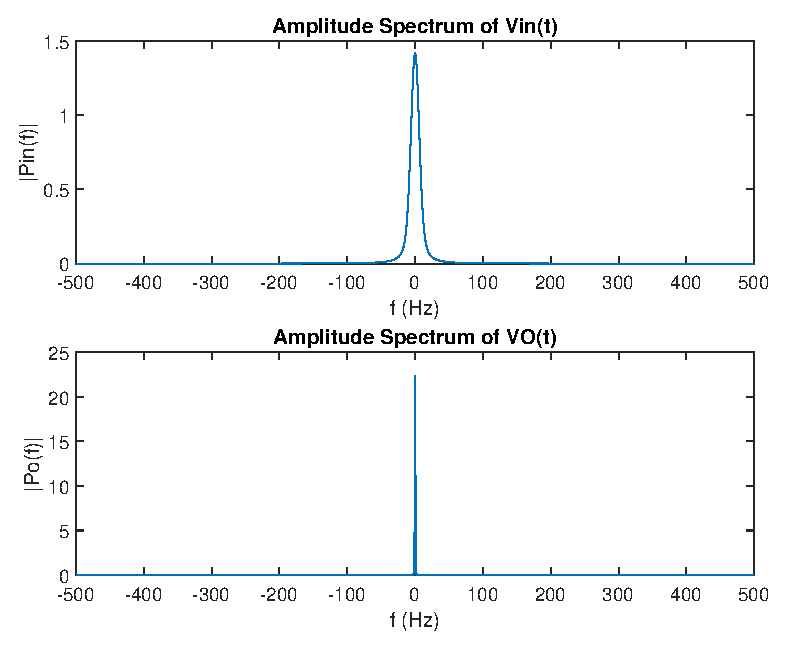
\includegraphics [width=4in]{main_23.eps}
\begin{par}
Figures 21 through 23, above, depict the input and output amplitude spectrum of the circuit as Cn changes. In Figure 21, \(C_n = 1 \times 10^{-15}F\), in Figure 22, \(C-n = 1 \times 10^{-6}F\) and in Figure 23, \(C_n = 1F\). Though these capacitance values are very different, there is not much difference in the amplitude spectrum with the only exception being the 0Hz response when \(C_n = 1F\).
\end{par} \vspace{1em}
\begin{par}
Next, we can also study the effect of dt on the simulation. Note, we do have to make some adjustments to the code to resonably scale the input signal to changes to dt.
\end{par} \vspace{1em}
\begin{verbatim}
C_n = 1e-5;
C(3,:) = [0 0 0 0 C_n 0 0 0];

for dt = [1e-4 1e-3 1e-2]

    varyTimeStep

    figNum = figNum + 1;

end
\end{verbatim}

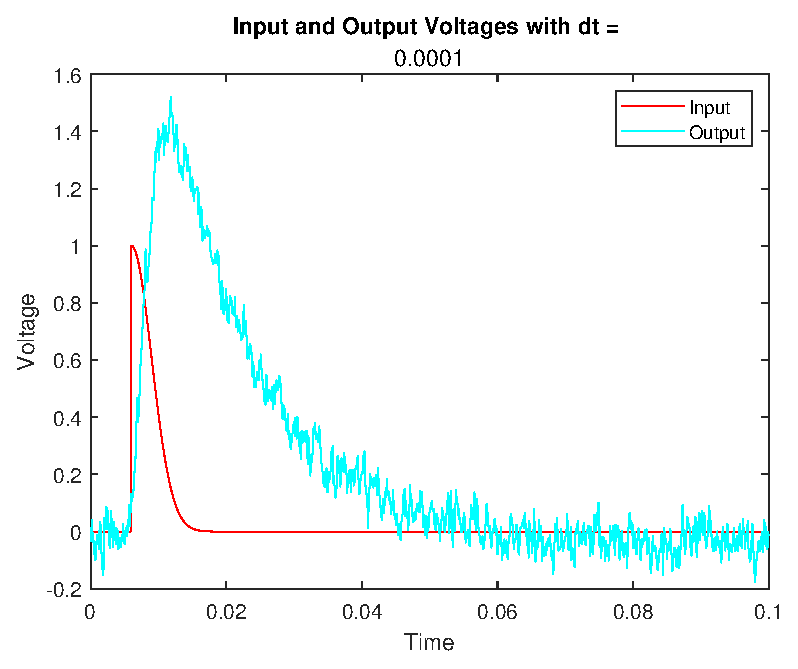
\includegraphics [width=4in]{main_24.eps}

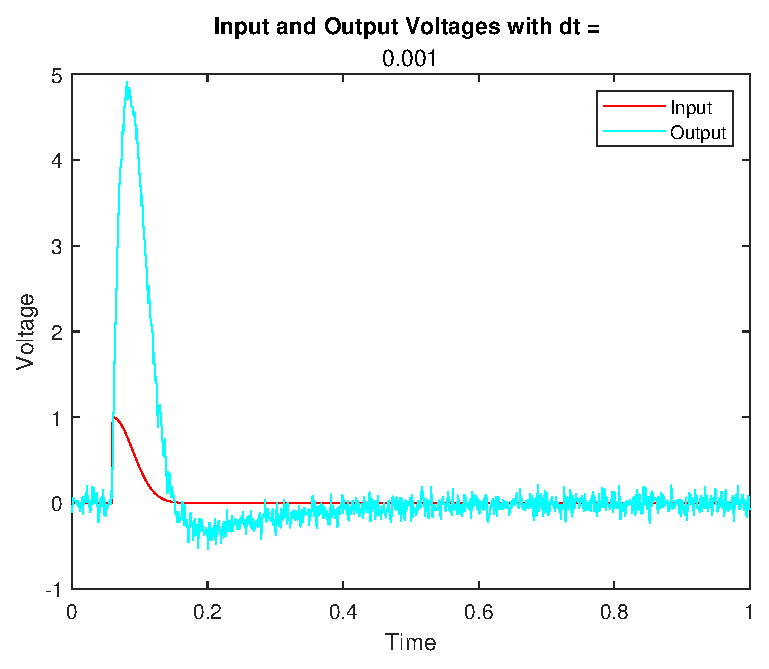
\includegraphics [width=4in]{main_25.eps}

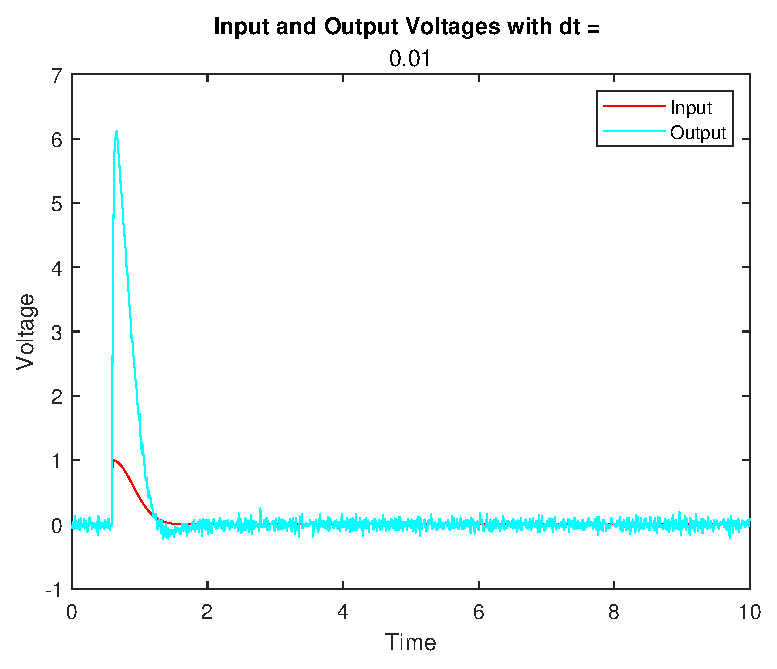
\includegraphics [width=4in]{main_26.eps}
\begin{par}
As mentioned earlier, dt effects the sampling frequency used to measure the input and output signals. Because a smaller dt means the signal is sampled more frequently, more noise is introduced to the output waveform, whereas at higher a dt there is more time between each sample creating a smoother looking curve as less noise is picked up.
\end{par} \vspace{1em}


\subsection*{Introducing a Non-Linear Transconductance}

\begin{par}
   By changing the current controlled voltage source to be a third order polynomial, more higher order terms would have to be added in addition to the C and G matricies - i.e.: 
\end{par} \vspace{1em}
\[C dV/dt + GV + AV^2 + BV^3 = F\]
\begin{par}
   Where I3 would be the only unknown associated with matricies A and B.
\end{par} \vspace{1em}


\end{document}

